\documentclass[10pt,twocolumn,letterpaper]{article}

\usepackage{cvpr}
\usepackage{times}
\usepackage{epsfig}
\usepackage{graphicx}
\usepackage{amsmath}
\usepackage{amssymb}

% Include other packages here, before hyperref.

% If you comment hyperref and then uncomment it, you should delete
% egpaper.aux before re-running latex.  (Or just hit 'q' on the first latex
% run, let it finish, and you should be clear).
\usepackage[breaklinks=true,bookmarks=false]{hyperref}

\cvprfinalcopy % *** Uncomment this line for the final submission

\def\cvprPaperID{****} % *** Enter the CVPR Paper ID here
\def\httilde{\mbox{\tt\raisebox{-.5ex}{\symbol{126}}}}

% Pages are numbered in submission mode, and unnumbered in camera-ready
%\ifcvprfinal\pagestyle{empty}\fi
\setcounter{page}{1}
\begin{document}
	
%%%%%%%%% TITLE\
\title{Term Project Report \\
Normal Map Estimation using Model Geometry and Texture \\
Team: Avengers }
\author{Jang Wonjong, Lee Dahun, Jacob Morton\\
	20140337, 20130221, 20172327\\
	Computer Science and Engineering, POSTECH\\
	{\tt\small}}

\maketitle
%\thispagestyle{empty}

%%%%%%%%% BODY TEXT
\section{Introduction}
\begin{figure}[t]
	\begin{center}
		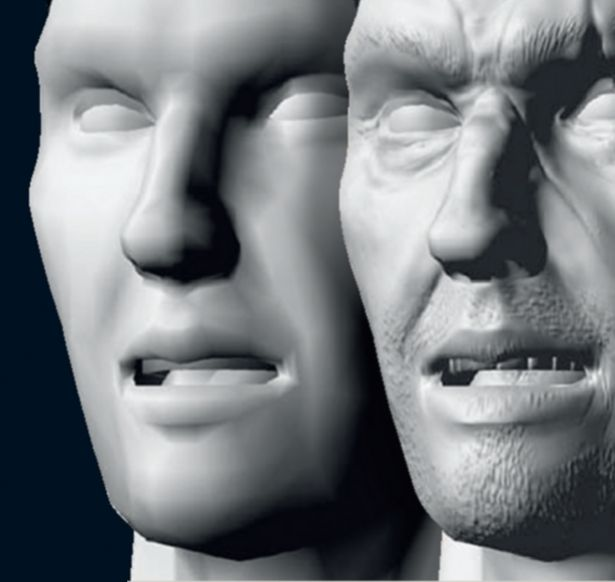
\includegraphics [scale=0.35] {image/face_normalmapping.jpg}
	\end{center}
	\caption{Example of a face model with \textbf{Left:} Geometry only, \textbf{Right:} Geometry + Normal Map}
	\label{fig:title}
\end{figure} 

\subsection{Motivation}
 There are several easy to use tools to generate 3D models geometry and texture, like 3D Studio Max, Maya, blender, and Photoshop. It is not too difficult to program or load these into OpenGL as well. The problem of using 3D geometry and Texture alone is that it can produce flat looking renderings, especially if the geometry is less detailed than the texture. This is typically the case, as texturing can hide simple geometry and flaws. There is more we can do with texture mapping than just wrapping the geometry with an RGB image. We can also add bump maps, normal maps, displacement maps, and even subsurface scattering to make the rendering more realistic. But these additional mappings are difficult to produce and are often hand-made or produced in multi-step procedures called baking. Baking is where a normal map is extracted from a high-resolution model and mapped onto a lower resolution model. Adding tuned normals to the texture can improve the perceptual quality of 3D reconstructed scenes and objects while being illuminated by a light source. We wish for there to be a simple automated procedure that can take an RGB picture with a geometric prior and produce a high-quality normal map.


\subsection{Project Description}
Inspired by Shape-From-Shading, we propose a tool for estimating a normal map from a given texture. We use geometric priors to extract interpolated surface normals that we will then refine. We use off-the-shelf Intrinsic Image Decomposition to estimate the albedo texture and remove shading from a single photograph. Given the albedo and interpolated normals we use Spherical Harmonics to first estimate the environment illumination and second compute a per-pixel normal map based on the diffuse surface illumination of the albedo. We can then apply this normal map in addition to the model and texture during the texturing process. We demonstrate this by using a fragment shader in OpenGL.




\subsection{Background}
This project requires knowledge in intrinsic image decomposition, Spherical Harmonics (SH), least-squares optimization, and normal mapping in OpenGL using fragment shaders. 
Intrinsic image decomposition is used to decompose an image into reflectance (albedo) and shading images. We can use spherical harmonics to estimate illumination parameters of the image scene. We can also refine the interpolated normals to better represent the surface geometry in the image. Spherical harmonics is a common method for illumination and geometric refinement.  The amount of energy a surface receives is proportional to the angle of a surface to a light source, which is related to the surface normal. We can use spherical Harmonics to measure this energy at each pixel on an image and determine the pixel's normal vector. Solving for normals and lighting is typically an intermediary step in SFS. We will use the first 3 bands of spherical harmonics, which is usually enough to represent reflectance sufficiently and hight orders are typically not used.
\begin{figure}[h]
	\begin{center}
		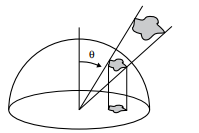
\includegraphics [scale=0.8] {image/energy.png}
	\end{center}
	\caption{light energy illuminated on a surface is proportional to cosine between the surface normal N and the unit vector towards the light source L}
	\label{fig:vgg-16}
\end{figure} 


\section{Development Environment}
\begin{table}[h]
	\begin{tabular}{ll}
		\textbf{Operating System:} &  Windows 10  \\
		\textbf{IDE:} &  MS Visual Studios 2017  \\
		\textbf{Libraries:} &  OpenGL, FreeGlut, GLEW, GLM,\\
		&chumpy
	\end{tabular}
\end{table}

\section{Overview}
\subsection{Intrinsic Image Decomposition}
We will use the geometric prior to extract the initial normal map $N_{ref}$. We also need a good approximation of the albedo texture $\rho(x,y)$, but it is difficult to acquire as we need an image without shading. We will pre-process the RGB image to remove shading $s(x,y)$ using widely available open-source Intrinsic Image Decomposition\cite{bell}. Intrinsic Image Decomposition is typically formulated as 
\begin{equation}
I(u,v) = \rho(u,v)s(u,v),
\end{equation}
Where $I(u,v)$ is the input raw image with shading from a lit environment. 
\begin{figure}[!h]
    \begin{center}
        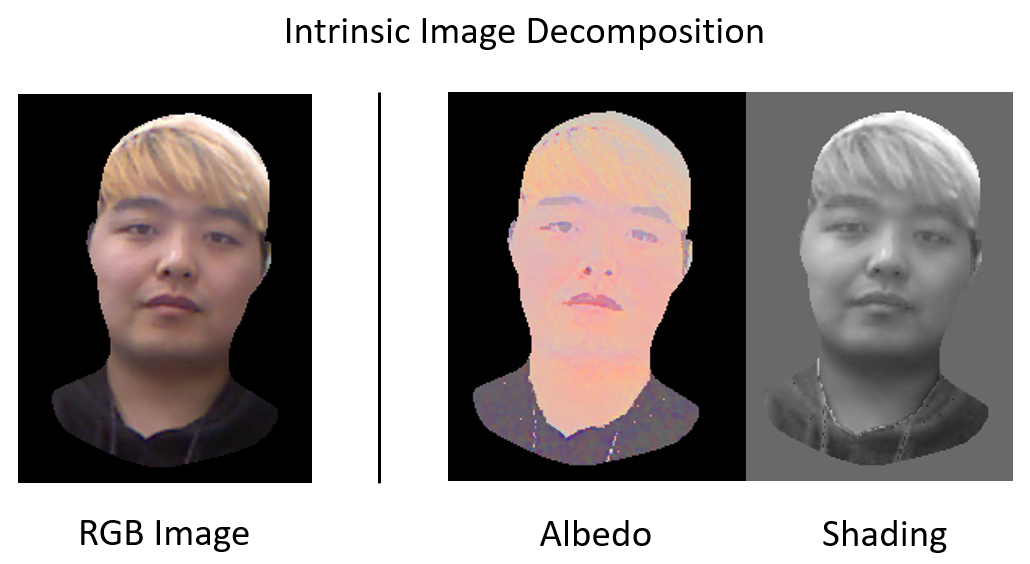
\includegraphics [scale=0.3] {image/intrinsic.png}
    \end{center}
    \caption{Decompose image $I$ into albedo $\rho$ and shading $s$}
    \label{fig:pipe1}
\end{figure} 

\subsection{Spherical Harmonics}
Spherical harmonics are a set of harmonic functions defined on the surface of a sphere. We will be using the real and Cartesian form of $2^{nd}$-order spherical harmonics. 
We will then Solve the least-squares problem to estimate lighting parameters $\hat{l}$ using SH and given $N_{ref}$ and $\rho(x,y)$ 
\begin{equation}
I = \rho \sum_{l,m} a_l L_m^l Y_m^l(N_{ref}),
\end{equation}
where $Y(n_x,n_y,n_z)$ is the Spherical Harmonics function in Cartesian space using the first 3 bands. After lighting has been estimated, we will solve for the normal map by refining $N_{ref}$ to produce $N$ using SH, the found lighting parameters $L$, and $\rho$,
\begin{equation}
I = \rho \sum_{l,m} a_l L_m^l Y_m^l(N).
\end{equation}
We will render the resulting normal map $N$ in OpenGL using a fragment shader. We represent a per-pixel formulation in uv-coordinates,
\begin{equation}
I(u,v) = \rho(u,v) \sum_{l,m} a_l L_m^l Y_m^l(n(u,v)).
\end{equation}
The set of real spherical harmonics functions in Cartesian space $Y_m^l$ for the first 3 bands are defined \cite{sfs} as 
\begin{equation}
\begin{split}
&Y_0^0 = c_0\\
&Y_1^{-1} = c_1 n_x\\
&Y_1^{0} = c_1 n_y\\
&Y_1^{1} = c_1 n_z\\
&Y_2^{-2} = c_2 n_x n_y\\
&Y_2^{-1} = c_2 n_x n_z\\
&Y_2^{0} = c_2 n_y n_z\\
&Y_2^{1} = \frac{c2}{2}(n_x^2 - n_y^2)\\
&Y_2^{2} = \frac{c2}{2\sqrt{3}}(3n_z^2 - 1),\\
\end{split}
\end{equation}
where coefficients $c_l$ are denoted as,
\begin{equation}
\begin{split}
&c_0 = \frac{1}{\sqrt{4\pi}}\\
&c_1 = \frac{\sqrt{3}}{\sqrt{4\pi}}\\
&c_2 = \frac{3\sqrt{5}}{\sqrt{12\pi}}.\\
\end{split}
\end{equation}
The Lambertian reflectance factors $a_l$ for the first three bands are defined as,
\begin{equation}
\begin{split}
&a_0 = \pi\\
&a_1 = \frac{2\pi}{\sqrt{3}}\\
&a_2 = \frac{2\pi}{\sqrt{8}}.\\
\end{split}
\end{equation}
The Illumination parameters $L_l^m$ are coefficients which represent multiple unknown light sources. In $2^{nd}$-order Spherical harmonics, we will need 9 (greyscale) or 27 (RGB) coefficients.

\subsection{Pipeline} 
\begin{figure}[!h]
    \begin{center}
        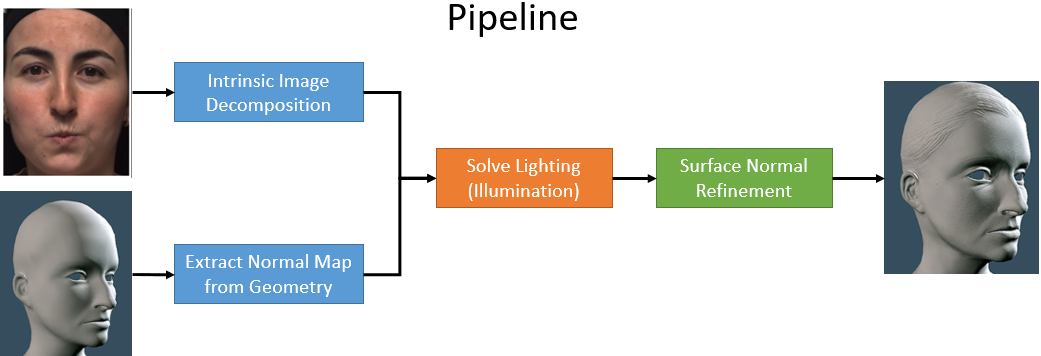
\includegraphics [scale=0.35] {image/pipeline.png}
    \end{center}
    \caption{Pipeline}
    \label{fig:pipe1}
\end{figure} 
Our pipeline begins with the pre-aquired geometry and an image $I$ with which to texture the 3D models. We first use intrinsic image decomposition to obtain the albedo $\rho$. Using the interpolated normals of the prior geometry as the prior normal map $N_{ref}$. Next we give the image $I$, albedo $\rho$, and the prior normal map $N_{ref}$ to our SH illumination and normal refinement solver, which outputs the refined normal map $N$. For face models we fit a parametric model (PCA) with facial landmarks\cite{pca} and project the model into image space to map uv-coordinates on the corresponding image.

\begin{figure}[!h]
    \begin{center}
        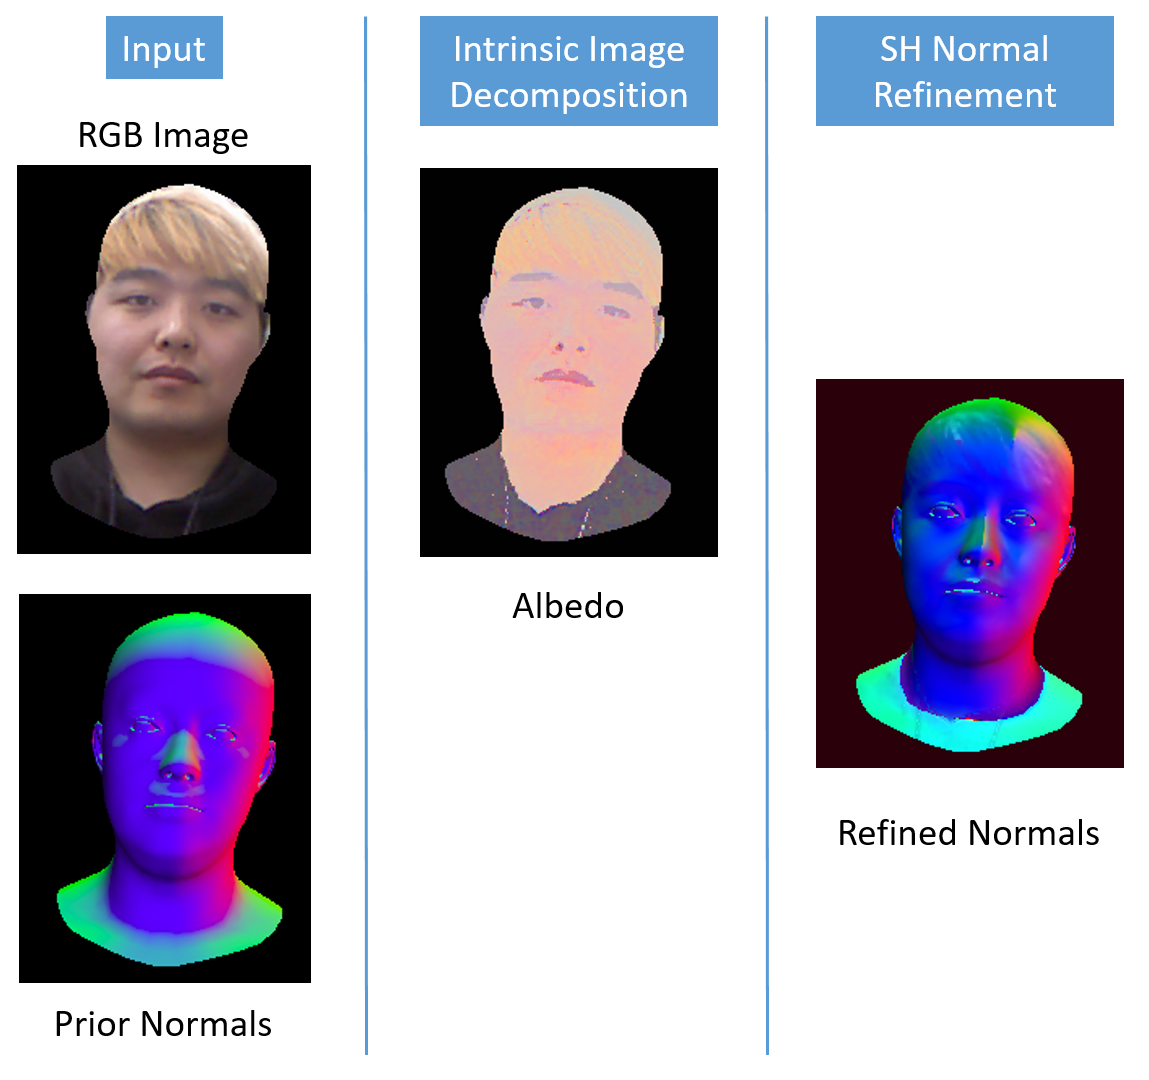
\includegraphics [scale=0.25] {image/refine_pipeline.png}
    \end{center}
    \caption{Refinement Pipeline: Inputs are Raw RGB image and Normals extracted from target geometry. Intrinsic Image Decomposition of Raw RGB image to get albedo. Solve for lighting using prior normal map and albedo. Refine Normals using albedo and solved lighting parameters.}
    \label{fig:pipe2}
\end{figure} 
We first solve for the unknown illumination parameters $L_l^m$ by minimizing the energy
\begin{equation}
\min_{L} I(u,v) - \rho(u,v) \sum_{l,m} a_l L_{lm} Y_{lm}(n_{ref}(u,v)).
\end{equation}
With illumination known, we next refine the prior normal map by minimizing
\begin{equation}
\min_{n} I(u,v) - \rho(u,v) \sum_{l,m} a_l L_{lm} Y_{lm}(n(u,v)).
\end{equation}
We use grayscale, as this has been shown\cite{sfs} to be sufficient for computing illumination and surface normals. 

\section{visualization}
    
\section{Results}
\subsection{Normal Refinement}
\subsection{Rendered Results}


\section{Team Member Roles}
See Table \ref{tab:roles}.
\begin{table}[!h]
	\begin{tabular}{l|l}
		\textbf{Name} & Roles \\
		\hline
		WonJong & Intrinsic Image Decomposition \\
		Dahun & Render Model, Texture, and Normal Map \\
		Jake & SH Normal Map Estimation \\
		\hline
	\end{tabular}
	\caption{Team Member Roles}
	\label{tab:roles}
\end{table}

\begin{thebibliography}{1}
	\bibitem{green} 
	R. Green.
	\textit{Spherical Harmonic Lighting: The Gritty Details}. 
	GDC 2003.
	
	\bibitem{dicky} 
	Rich Forster.
	\textit{Spherical Harmonics for Beginners}. 
	https://dickyjim.wordpress.com/2013/09/04/spherical-harmonics-for-beginners/
	
	
	\bibitem{igor} 
	Igor Goldvekht. 
	\textit{Shape-From-Shading}. 
	https://github.com/IgorGee/Shapes-From-Shading
    
    
    \bibitem{bell} 
    Sean Bell, Kavita Bala, Noah Snavely
    \textit{Intrinsic Images in the Wild” ACM Transactions on Graphics}
    SIGGRAPH 2014.
    
    \bibitem{sfs} 
    Ira Kemelmacher-Shlizerman, Member, IEEE, and Ronen Basri, Senior Member, IEEE \textit{3D Face Reconstruction from a Single Image Using a Single Reference Face Shape}
    IEEE TRANSACTIONS ON PATTERN ANALYSIS AND MACHINE INTELLIGENCE, VOL. 33, NO. 2, FEBRUARY 2011.
    
    \bibitem{pca} 
    Volker Blanz, Thomas Vetter
    \textit{A Morphable Model For The Synthesis Of 3D Faces}
    SIGGRAPH 1999
    
\end{thebibliography}

\end{document}
